\documentclass[discrete.tex]{subfiles}

\begin{document}
  \section{Двоичный поиск и неравенство Крафта}

  \begin{definition}[схема дихтомического (двоичного) поиска]
    Разыскиваем на прямой линии отрезок, соответствующий нужному значению индекса, разбиваем область поиска на две части и устанавливаем, в какой лежит интересующий нас индекс.

    Затем повторяем действие для оставшейся части, пока не найдем часть, содержащую только одно значение индекса.
  \end{definition}

  \begin{theorem}
    Для того чтобы набор из целых чисел $s_1,...,s_m$ мог быть набором длин путей в схеме с m исходами необходимо и достаточно, чтобы:
    \[\sum_{i \in 1:m} 2^{-S_i} \leqslant 1,\q \text{$S_i$ - числа из набора}\]
  \end{theorem}

  \begin{proof}
    (Необходимость $\Ra$):

    Рассмотрим поисковую схему - двоичное дерево $T$ с $m$ листьями, сопоставим каждой вершине k, находящейся на расстоянии t от корня, $a_k=2^{-t}$. То есть если $r_0$ - корень $\Ra a_{r_0} = 1$. Значит мы должны доказать: \[a_{r_0} \geq \sum_{k \in F} a_k, \text{ где F - мн-во листьев}\]

    Для каждого не-листа $k \in M \setminus F$ следует:
    \[(*)\qq a_k \geqslant \sum_{r \in \next(k)} a_r,\text{ где $\next(k)$ - мн-во прямых потомков k}\]
    В случае двух вершин неравенство выполняеся как равенство. В случае одной - как строгое неравенство. Суммируя неравенства (1) по $M \setminus F$ получаем:
    \[\sum_{k \im M \setminus F} a_k \geq \sum_{r \im M \setminus \{r_0\}} a_r\]
    Сокращение обзих слагаемых (промежуточных частях неравенств) и дает искомое

    (Достаточность $\La$):

    Взяв $m$ чисел $s_k$, удовлетворяющих условию теоремы, расположим их в порядке возрастания. Определим, как и раньше, числа $a_k = 2^{-s_k}$ и положим:
    \[b_1 = 0;\qq b_{k+1} = b_k + a_k,\qq k>1\]
    \[P_a = 0,07 \q P_b = 0,31 \q P_c = 0,35 \q P_d,27\]
    Рассмотрим последовательности из нулей и единиц $t_k$, являющиеся двоичными представлениями дробей $b_k$, в каждой такой дроби $b_k$ возьмем первые $s_k$ знаков. Покажем, что никакая из последовательностей $t_k$ не является началом другой такой последовательности.

    Так как длины последовательностей $t_k$ не убывают с ростом k, нам достаточно показать, что никакая последовательность $t_k$ не является началом последовательности с большим номером. Так как дроби $b_i$ возрастают, то $b_k < b_{k+1} < ... < b_m \leq 1$. Обозначим через $b_r^{(k)}$ число, получающееся из $b_r$, отсечением первых $s_k$ цифр. Очевидно, что для таких "урезаний"{} сохраняется то же неравенство, хотя и нестрогое $b_k < b_{k+1}^{(k)} \leq ... \leq b_m^{(k)}$. При этом первое из неравенств осталось строгим, так как $b_k + a_k = b_{k+1} = b_{k+1}^{(k)}$. Следовательно, начало $t_k^{(k)}$ никакой дроби $b_r$ не совпадает с $t_k$ при $r>k$.

    Далее, любой набор последовательностей $t_k$, из которых ни одна не является началом другой, задает некоторую процедуру поиска. Действительно, рассмотрим полное двоичное дерево с достаточно большим числом этажей и наложим на это дерево все последовательности $t_k$, трактуя каждую из них как путь от корня, который идет влево, если очередной элемент последовательности равен 0, и вправо - для единицы. В силу сделанного предположения ни одна из вершин, соответствующих концам последовательностей, не лежит на какой-либо другой последовательности как промежуточная вершина.
  \end{proof}

  \begin{example} \
    \begin{tabular}{c|c|c|c}
      & a_i & b_i & \\
      2 & 0.010..0 & 0.00000 & 00\\
      2 & 0.010.. & 0.01000 & 01\\
      3 & 0.001.. & 0.100|00 & 100\\
      3 & 0.001.. & 0.101|00 & 101\\
      3 & 0.001.. & 0.110|000 & 110\\
      5 & 0.00001 & 0.111000 & 11100\\
      5 & 0.00001 & 0.11101 & 11101\\
      5 & 0.00001 & 0.11110 & 11110\\
      6 & 0.000001 & 0.111110 & 111110\\
      6 & 0.000001 & 0.111111 & 111111
    \end{tabular}

    \begin{figure}[H]
        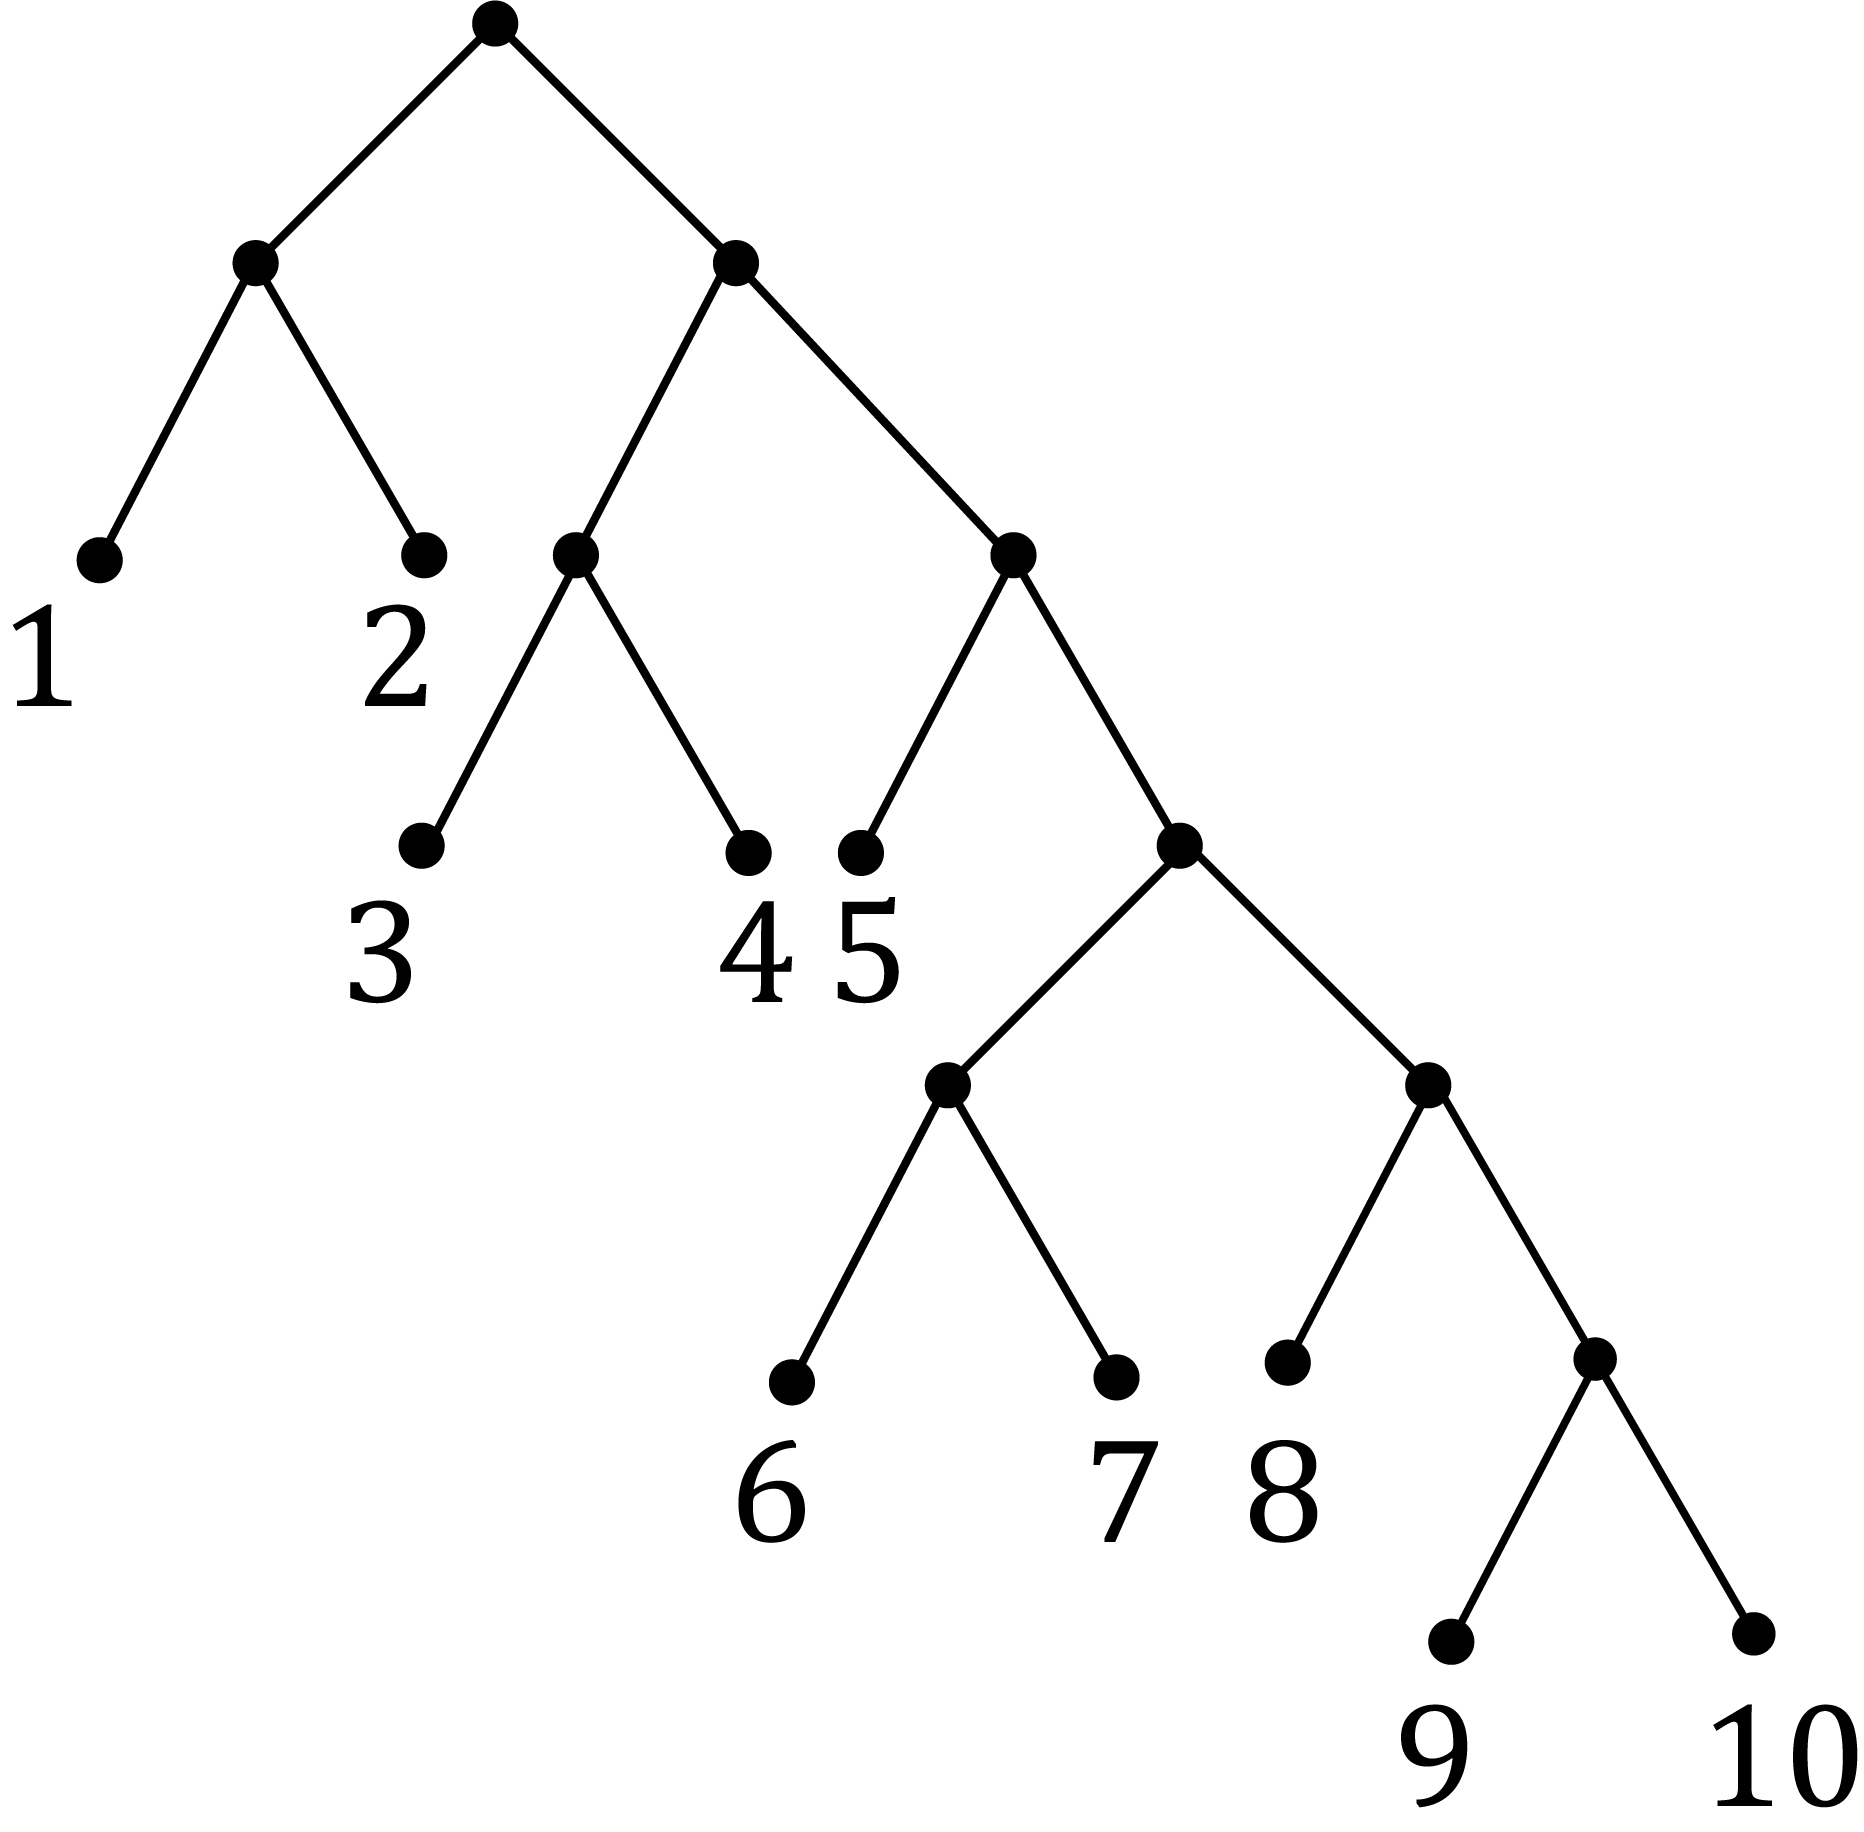
\includegraphics[width=10cm]{pics/18_1.png}
        \centering
    \end{figure}
  \end{example}
\end{document}
